%% Copyright (C) 2008 Johan Oudinet <oudinet@lri.fr>
%%  
%% Permission is granted to make and distribute verbatim copies of
%% this manual provided the copyright notice and this permission notice
%% are preserved on all copies.
%%  
%% Permission is granted to process this file through TeX and print the
%% results, provided the printed document carries copying permission
%% notice identical to this one except for the removal of this paragraph
%% (this paragraph not being relevant to the printed manual).
%%  
%% Permission is granted to copy and distribute modified versions of this
%% manual under the conditions for verbatim copying, provided that the
%% entire resulting derived work is distributed under the terms of a 
%% permission notice identical to this one.
%%  
%% Permission is granted to copy and distribute translations of this manual
%% into another language, under the above conditions for modified versions,
%% except that this permission notice may be stated in a translation
%% approved by the Free Software Foundation
%%  
\chapter{Etat de l'art} \newline{}
\section{Préliminaires}    
\label{sec:prelimin} 
\subsection{Le cloud computing} 
L’expansion d’Internet a permis l’émergence du   cloud computing. 
La définition la plus répandue et acceptée est celle du \cite{NIST}. Le NIST définit  le  Cloud computing, comme un modèle Informatique qui permet un accès facile et à la demande par le réseau à un ensemble partagé de ressources informatiques configurables (serveurs, stockage, applications et services) qui peuvent être rapidement provisionnées et libérées par  un minimum d’efforts de gestion ou d’interaction avec le fournisseur du service.
D’un point de vue technique,  le cloud est la réunion  de plusieurs concepts informatiques dont les  principaux sont le Grid computing \cite{Grid} et la virtualisation.  Le Grid computing permet l’agrégation des ressources distribuées. La virtualisation quant à elle assure les  trois propriétés suivantes :
\begin{itemize} 
 \item  \textbf{Mutualisation des ressources}: la virtualisation permet d’affecter les ressources d’une même machine à plusieurs applications;
 \item  \textbf{ Abstraction de la localisation}: L’utilisateur a accès à une machine virtuelle complète qui  se trouve  quelque part  sur un serveur, comme si elle lui était locale;
 \item  \textbf{Elasticité} : Il est possible d’allouer des ressources supplémentaires à une application en fonction des besoins.
\end{itemize}\newline

 On distingue en outre, plusieurs types de cloud: 

 \begin{itemize} 
 \item  \textbf{Cloud privé}: L’infrastructure Cloud est utilisée par une seule organisation. Elle peut être gérée par l’organisation ou par une tierce partie (Ex: OpenStack \cite{openstack});
 \item  \textbf{ Cloud public}: L’infrastructure Cloud est partagée par plusieurs organisations pour les besoins d’une communauté qui souhaite mettre en commun des moyens (sécurité, conformité, etc..);
 \item  \textbf{Cloud hybride} : L’infrastructure Cloud est composée d’un ou plusieurs modèles  ci-dessus qui restent des entités séparées. 
\end{itemize}\newline


Structurellement, trois modèles de services peuvent être offerts sur le Cloud:              
   
\begin{itemize} 
 \item  \textbf{Software-as-a-Service (SaaS)}: Ce modèle de service est caractérisé par l’utilisation d’une application partagée qui fonctionne sur une infrastructure Cloud. L’utilisateur accède  à l’application par le réseau au travers de divers types de terminaux (souvent via un navigateur Web). 
 \item  \textbf{ Platform-as-a-Service (PaaS)}: l’utilisateur a la possibilité de créer et de déployer sur une infrastructure Cloud PaaS ses propres applications en utilisant les langages et les outils du fournisseur. L’utilisateur ne gère pas ou ne contrôle pas l’infrastructure Cloud sous-jacente (réseaux, serveurs, stockage) mais contrôle l’application déployée et sa configuration.
 \item  \textbf{Infrastructure-as-a-Service (IaaS)} :L’utilisateur loue des moyens de calcul et de stockage, des capacités réseau et d’autres ressources indispensables (partage de charge, pare-feu, cache). L’utilisateur a la possibilité de déployer n’importe quel type de logiciel incluant les systèmes d’exploitation.  
\end{itemize} \newline
\par 
L’un des concepts majeurs associés au cloud est la multi-tenancy ou la possibilité d'avoir des infrastructures multi-locataires.  La multi-tenancy permet à des entités d’exécuter simultanément  des instances d’une même application, d’un même réseau ou d’une même plateforme.
Nous nous intéressons maintenant à l’architecture  des caches des processeurs qui constituent le principal vecteur d’attaque dans notre étude. 

\subsection{Architecture et fonctionnement des caches}   
L’avènement des nouvelles générations de processeur telles que les multi-cœurs imposent des architectures plus performantes. C’est ce qui a favorisé le concept de \textbf{cache}. Les caches ou mémoires cache sont des mémoires très rapides mais de faible capacité de stockage servant à  stocker des données temporaires. Les caches ont été instaurés dans les architectures matérielles  des processeurs afin de limiter l’impact des temps d’accès à la mémoire depuis le processeur vers la mémoire centrale et vice-versa. Les caches fonctionnent sur deux principes fondamentaux : \textbf{la localité spatiale} et \textbf{ localité temporelle}. La localité spatiale est le fait que le processeur a tendance à accéder aux données proches des données accédées précédemment. La localité temporelle consiste au fait que le processeur a également tendance à accéder à une donnée accédée récemment. Le cache est divisé en blocs de même taille appelés \textbf{lignes de caches} contenant des blocs de  lignes de mot de la mémoire centrale appelées\textbf{pages}. La correspondance entre les lignes de caches et les pages se fait de différentes manières. On distingue alors 3 types de caches: 
\begin{enumerate}
 \item  \textbf{Les caches à  correspondance directe}: Chaque page de la mémoire correspond à une unique ligne dans le cache. Cette méthode à l’avantage de permettre un accès rapide à la ligne de cache  car on sait directement où elle se trouve. Cependant cette méthode s’avère peu efficace en pratique car on a souvent les mêmes données accédées tandis que les autres restent inutilisées.
 \item  \textbf{Les caches associatifs}: Dans ce type de cache, chaque page peut être chargée dans n’importe quelle ligne de cache. L’avantage ici c’est qu’on a un accès rapide au cache. Le principal goulot d’étranglement est la recherche d’une donnée préalablement dans le cache ce qui peut nécessiter de parcourir toutes les lignes.
 \item  \textbf{Cache way-associatif}: c’est un compromis entre les deux types précédents de cache. Dans ce cas, le cache est subdivisé en k blocs de taille égale appelé \textbf{sets}, chaque bloc comprenant un certain nombre \textit{w} (\textbf{way}) de lignes de cache. Chaque  page appartient correspond à un unique set, mais l’accès dans le set  se fait de manière aléatoire. C’est ce type de cache qui est le plus utilisé dans les architectures actuelles.
\end{enumerate}
\par

Ces architectures proposent une hiérarchie de cache organisée en plusieurs niveaux. Un niveau L1 plus près de la mémoire avec un accès rapide et une  taille moins importante généralement scindé en deux parties : une partie données (D), et une partie  instructions (I). On a en outre le niveau L2 qui est un peu moins rapide que  le niveau L1 mais plus grand en espace. Finalement, certains processeurs disposent d’un troisième niveau L3 de cache plus grand en espace mais le moins rapide.  Pour chercher les données, on commence   d’abord par le cache L1 ; dans ce cas on a un cache hit si la donnée est trouvée sinon on a un cache miss et on continue la recherche dans le cache L2 voire le cache  L3 au besoin.

\begin{figure}[h!]
   \begin{minipage}[b]{0.50\linewidth}
      \centering 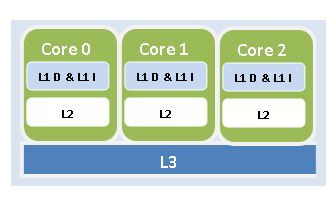
\includegraphics[scale=0.68]{cache.jpg}
      \caption{\it Architecture classique des caches}
   \end{minipage}\hfill
   \begin{minipage}[b]{0.50\linewidth}   
      \centering 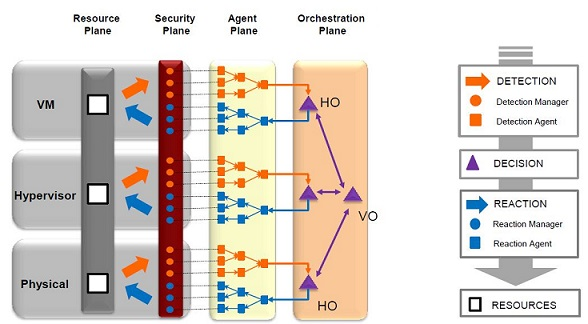
\includegraphics[scale=0.5]{vespa.jpg}
      \caption{Architecture du framework Vespa \cite{Vespa}}       
   \end{minipage}
\end{figure}      
% 
% \begin{figure}[H]
%   \begin{flushleft} 
%   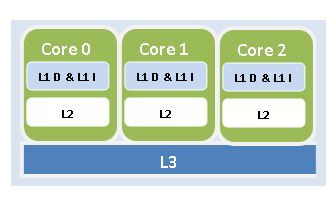
\includegraphics[scale=0.5]{cache.jpg}
%    \caption{Architecture classique des caches}
%   \end{flushleft}
% \label{Cache}
% \end{figure}
% 
% \begin{figure}[H]
% \begin{flushright}
% 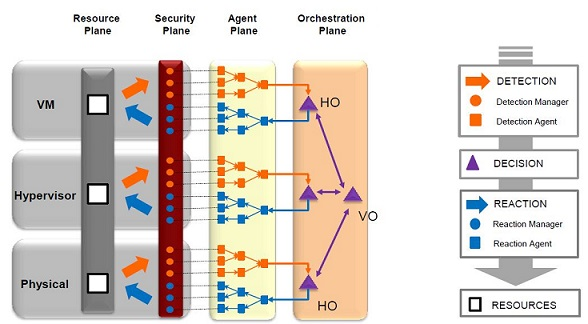
\includegraphics[scale=0.5]{vespa.jpg}
% \caption{Architecture du framework Vespa \cite{Vespa}}
% \end{flushright}
% \label{vespa}
% \end{figure}
% 
% \begin{figure}
%     \begin{minipage}[t]{0.84\textwidth}
%         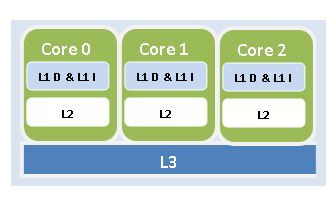
\includegraphics[width=6cm]{cache.jpg}
%     \end{minipage}  
%     \begin{minipage}[t]{0.15\textwidth}
%         \begin{flushright}
%         \includegraphics[width=\textwidth]{vesps.jpg}
%         \end{flushright}
%     \end{minipage}
% \end{figure}



\subsection{Le Framework de sécurité autonome VESPA} 
\textbf{ VESPA (Virtual Environments Self-Protecting Architecture)} \cite{Vespa} a été développé à Orange Labs Issy-les-Moulineaux dans le cadre du projet OpenCloudWare \cite{OpenCloudWare}. VESPA est une architecture de protection d'automatisation de la sécurité qui a pour but d’apporter une solution au manque d’outil de protection autonomique.  La sécurité autonome fait partie intégrante de \textbf{ <<l’autonomic computing>>} promue par IBM \cite{ibm}qui consiste à avoir des systèmes qui s’auto-administrent, s’auto-réparent et s’auto-protègent. La sécurité autonomique  a récemment connu un intérêt pour la plupart des fournisseurs de cloud et des géants d’internet comme une solution possible à l’épineux problème qu’est la protection des infrastructures de cloud computing.
\par L’approche autonomique propose une gestion plus simple et plus efficiente. En outre, toutes les solutions proposées dans le passé ne sont pas adaptées à l’environnement de cloud. En effet, elles souffrent du manque de politiques de sécurité flexibles, de l’absence de sécurité multicouche et  des architectures non extensibles.  VESPA  apporte une solution à  ces limitations. VESPA  a une architecture d’autoprotection,  qui se base sur des politiques de sécurité sûres et robustes. Il régule la sécurité sur deux niveaux, à l’intérieur ainsi qu’à travers les couches de l’environnement cloud. Son architecture extensible lui  permet d’intégrer simplement d’autres composants de détection et de réaction.  
          
\section{Attaques par canaux auxiliaires} 
\subsection{Définition et classification}
     
Les prouesses de la cryptographie moderne ont permis la conception d’algorithmes mathématiquement  prouvés robustes et sûrs (\cite{Kocher}, \cite{Rsapaper}). Ces algorithmes suffisent  donc théoriquement  pour assurer  la confidentialité, l’intégrité, l’authenticité des données sensibles d’une  personne ou d’une entité. Bien que ces algorithmes soient sûrs, leurs implémentations logicielles ou matérielles peuvent être sujettes à des attaques dites attaques par \textbf{canaux cachés}. Une attaque par canaux cachés  utilise des moyens de communication qui normalement  ne sont pas prévus  pour laisser fuir les informations \cite{Covert}(ex. écrire et vérifier si  un fichier verrouillé pour convenir un bit « 1 » ou « 0 »). On a un processus \textit{émetteur} et un autre processus \textit{récepteur} . L’émetteur pourrait bien être  un programme malveillant préalablement installé sur le système de la victime  par l’attaquant après avoir compromis ce système et le récepteur un processus non privilégié. \newline{}

\par

Une attaque par \textbf{canal auxiliaire} est un type particulier d’attaque par canaux cachés. Dans ce type d’attaque, Il n’y a pas de compromission des mécanismes de sécurité. En effet, ces attaques se font d’abord par l’analyse fine de  la consommation électrique, de l’émanation électromagnétique  ou bien du temps pendant  l’exécution  d’un  système cryptographique. L’exploitation des résultats de la phase d'analyse rend l’attaquant  capable   de  recouvrir des bits de clés de chiffrement de certains algorithmes. 
Il existe deux grandes familles d’attaques par canaux auxiliaires selon \cite{sidechannelattack}: \textbf{les attaques internes} et\textbf{les attaques externes}. Dans une attaque interne, l’espion contrôle soit  un processus ou une application dans un environnement partagé tel que  le cloud. Ce type d’attaques est basé sur  l’analyse de l’utilisation d’une ressource matérielle partagée comme le cache des processeurs ou les disques durs. Par contre dans une attaque externe, l’attaquant  réussit  au préalable à posséder physiquement un système informatique avant de réaliser l’attaque. \newline{}

\par


On distingue en outre plusieurs manières d’effectuer les attaques dont certaines sont communes aux deux familles d’attaques mentionnées plus haut.Il s’agit :
\begin{enumerate}
 \item  Des attaques basées sur \textbf{les accès aux ressources}: L’attaquant inspecte  l’état de la ressource partagée lorsque la victime est en fonctionnement et effectue ces analyses à la suite. Ces attaques sont le plus souvent réalisées sur  \textbf{les caches} ou \textbf{les prédicteurs de branche}. Ces attaques sont les plus représentatives dans le cloud puisque cette technologie se base sur le partage de ressources. 
 \item Des attaques basées sur \textbf{ le temps d’exécution}: Dans ce cas de figure, l’attaquant s’appuie sur le temps d’exécution pour compromettre le système. En effet, il exécute plusieurs fois le programme en  fournissant des données différentes en entrée  et à chaque exécution enregistre le temps mis. Il s’ensuit une analyse de ces temps pour inférer les clés de sécurité.
 \item Des attaques basées sur \textbf{ les traces}: Ce type d’attaque se base sur l’évaluation de  la consommation énergétique des systèmes cryptographiques. Il s’agit en fait de mesurer le courant électrique consommé par les circuits électroniques composant ces systèmes lorsqu’ils exécutent des programmes cryptographiques.  Une trace est alors un ensemble de mesures de consommation effectuées pendant le déroulement d’une opération. L’analyse des courbes obtenues et des niveaux de courant enregistrés sert à la conjecture des bits  des clés. Ces attaques sont le plus souvent effectuées sur des composants embarqués comme les cartes à puces. \par Par ailleurs, on trouve deux  sous-classes dans cette famille \cite{Kocher}:
  \begin{itemize}
   \item  \textbf{La SPA (Simple Power Analysis)}: Dans cette sous-classe, les données  recueillies après la phase d’analyse sont directement  exploitées et interprétées.
   \item  \textbf{La DPA (Differential Power Analysis)}: Ici par contre on effectue l’analyse différentielle de la consommation. En fait, on combine les résultats de la phase d’analyse avec  des méthodes statistiques pour l’extraction des clés.
  \end{itemize}
Ces deux sous-classes d’attaques sont facilement automatisables et ne nécessite pas la connaissance de l’architecture de la plateforme cible.
\end{enumerate}\newline


Dans le cloud la ressource matérielle la plus utilisée comme vecteur d’attaques par canaux auxiliaires  est le cache. Ceci étant, notre présente étude se limitera aux attaques basées \textbf{les accès aux caches}
\subsection{Attaques par canaux auxiliaires dans le cloud}
\subsubsection{Attaques visant les caches L1 et L2}
Les attaques par canaux auxiliaires existaient bien avant l’apparition du cloud computing. Les attaques dans le cloud sont rendues possibles grâce au concept de multi-tenancy. La première étude qui a révélé la vulnérabilité  des plateformes de cloud computing est \cite{Ris2009}.L’attaque  a été menée sur  la plateforme de cloud public Amazon Web Services \cite{amazon} avec l’hyperviseur Xen \cite{xen}. Il faut noter qu’un hyperviseur est un logiciel système qui assure le lancement, la gestion et l’approvisionnement des machines virtuelles dans une plateforme cloud. Dans le cas de l’hyperviseur XEN, on distingue une machine virtuelle particulière et  privilégiée dénommée Dom0 qui agit comme orchestrateur des autres machines virtuelles et assure les fonctions de gestion. L’attaque s’est faite selon deux étapes distinctes:
\begin{enumerate} 
\item la première étape  a permis à  l' attaquant de faire une cartographie des adress internet et lancer sa machine virtuelle(VM) sur une même plateforme physique (CPU, cœur)  que la VM cible, ce qui est  connu sous le terme de \textbf{co-résidence}. Deux machines virtuelles sont considérées co-résidentes si l’une des trois conditions suivantes est vérifiée:
\begin{itemize}
 \item Elles ont des adresses internes proches;
 \item On a des latences réseau faibles entre les machines;
 \item Leurs adresses correspondent en partie à l’adresse  IP de Dom0;
\end{itemize}
\item La seconde étape consiste à l’exploitation de la co-résidence. L’attaquant utilise pour ce faire, la méthode du \textbf{PRIME TRIGGER AND PROBE}  qui est une variante de la méthode  du \textbf{ PRIME AND PROBE}.
\end{enumerate}

Le fonctionnement de la méthode du  \textbf{ PRIME AND PROBE} \cite{Osvik} est le suivant:
\begin{enumerate}
 \item L’attaquant remplit une ou plusieurs lignes du cache avec des données aléatoires;
 \item Puis il laisse la main à la victime pour qu’elle puisse s’exécuter;
 \item L’attaquant charge alors ces mêmes  données dans ces  mêmes lignes  de cache et mesure le temps mis pour le chargement.	
\end{enumerate}

\begin{figure}[h!]
      \centering 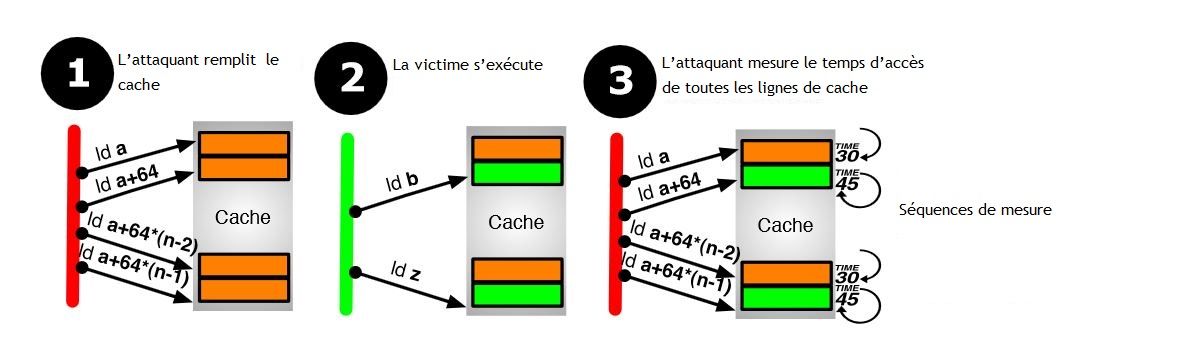
\includegraphics[scale=0.6]{prime-probe-tw.jpg}            
      \caption{\it Fonctionnement du PRIME AND PROBE \cite{TimeWarp} }
\end{figure}     

Le temps de chargement est parfaitement corrélé à l’accès de la victime au cache. Un temps de chargement d’une ligne de cache plus grand indique  que cette ligne de cache a été accédée par la victime et ses données ont été éjectées du cache. Par contre, une faible durée montre que la partie du cache L2 concernée est restée intacte. Ces mesures  ont permis  de mesurer le trafic d'un serveur Web et de détermier le lien entre les pics de  charge du cache  et les frappes des touches du clavier. En conclusion, il faut noter que  ces attaques ne sont pas assez robustes, car elles génèrent assez de faux-positifs et on ne peut qu’obtenir certaines parties des clés de chiffrement. Néanmoins cette étude, a ouvert  ce domaine de recherche et  a servi de tremplin aux futures attaques par canaux auxiliaires. \newline{}

\par 

Ainsi, une nouvelle attaque  a été montée\cite{Zhang2012}. L'attaque s'est déroulée des systèmes \textbf{ SMP (Symetric multiprocessing)}avec l’hyperviseur Xen. Le SMP est un mode de fonctionnement particulier où tous les processeurs exécutent en parallèle le même calcul.L’hypothèse  de base est  que l’attaquant est incapable d’exploiter des vulnérabilités logicielles qui lui permettent de prendre contrôle de l’infrastructure physique et n’a aucune  connaissance du logiciel cryptographique qu’exécute la victime. L’attaque  vise à recouvrir les clés de l’algorithme de chiffrement ElGamal\cite{ElGamal}. L'attaquant a d'abord obtenu la co-résidence avec la victime et a mesuré par la suite ,l'activité du cache  L1 ,grâce à la méthode du \textbf{PRIME AND PROBE}.  

\par

Il faut noter que pour qu’une attaque par canaux auxiliaires soit réalisable, il faudrait que l’attaquant ait la possibilité de \textbf{ préempter} régulièrement la victime. Lors de la mise en œuvre de la phase de mesure, l'attaquant a donc  été confronté à des difficultés  puisque le \textbf{ multithreading} n’était pas activé. Le multithreading est la capacité de lancer plusieurs threads dans une unité de calcul (cœur par exemple) d’un processeur. Le \textbf{ multithreading  temporel}se fait quand les threads s’exécutent tour à tour et \textbf{ le multithreading simultané } quand les threads s’exécutent simultanément. L'attaquant a réussi à contourner cet obstacle  en se basant sur le comportement de l’hyperviseur Xen consistant à donner la priorité d’exécution aux  \textbf{ processeurs virtuels (Virtual CPU)}  recevant des \textbf{interruptions}.L'attaquant peut régulièrement préempter la victime  en lançant des \textbf{ interruptions entre les processus}.  L'étape  finale est donc \textbf{ la classification}  des mesures de l'activité du cache et la détection des faus positifs grâce aux classificateurs utilisés dans les techniques d’apprentissage automatique \textbf{(Machine Learning)}. Grâce à cette technique, l’algorithme de chiffrement Elgamal \cite{ElGamal} a été cassé. Cette attaque est la première attaque par canaux auxiliaires dans le cloud la plus robuste avec une très fine granularité. \newline

\newline{}
\par 

Une autre méthode d'attaque est la technique  de l'\textbf{EVICT + TIME} \cite{Osvik} qui s'effectue également en trois étapes:
\begin{enumerate}
 \item D'abord, le programme de la victime est lancé et son temps d'exécution est mesuré;
 \item ensuite, l'attaquant évince un set spécifique du cache;
 \item finalement, il mesure de nouveau le temps d'exécution de la victime.
\end{enumerate}
Si le temps d'exécution croit, la victime a éventuellement accédé au cache.
Toutes  ces attaques  que nous avons présentées ne se basent que sur la mesure de l’activité des caches  L1 et L2. Nous verrons donc dans ce qui suit des attaques qui exploitent les caches L3.
\subsubsection{Attaques visant les caches L3}

Les caches L3 étant les caches les moins rapides d’accès,  très peu d’attaques utilisant ce cache comme vecteur d’attaque aboutissent. Une attaque ayant eu du succès est celle de Yuval et al. \cite{Yuval}. Les auteurs ont montré la possibilité de monter une attaque par canaux auxiliaires dans le cloud au travers du cache L3.  Leur attaque tire parti de la politique  \textbf{ déduplication de mémoire} qui est une technique de partage des pages dans les architectures \textbf{ Intel x86} qui assure la performance en  évitant  la réplication de copies de même contenu et la réduction des traces de la mémoire. 


\begin{figure}[h!]
   \begin{minipage}[b]{0.50\linewidth}
      \centering 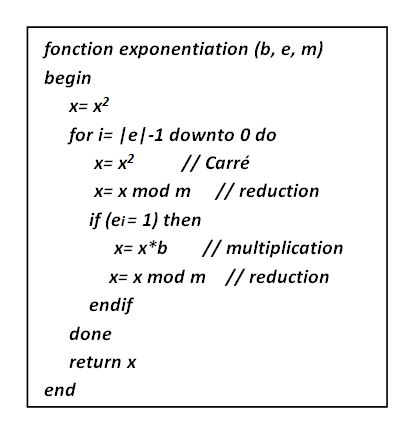
\includegraphics[scale=0.68]{exponentiation.jpg}
      \caption{\it Algorithme d'exponentiation}
   \end{minipage}\hfill
   \begin{minipage}[b]{0.50\linewidth}   
      \centering 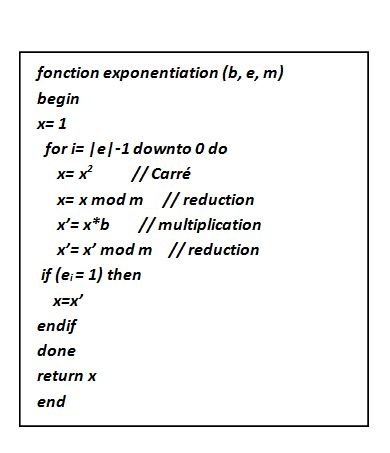
\includegraphics[scale=0.7]{exponentiation-new.jpg}
      \caption{Algorithme d'exponentiation réécrit}       
   \end{minipage}
\end{figure}    

Elle introduit  par ailleurs une nouvelle méthode d’attaque, le  \textbf{ FLUSH AND RELOAD} qui est une variante de la méthode PRIME AND PROBE.  Elle nécessite que la victime et l’attaquant partagent la hiérarchie de cache, et les pages de la mémoire et doivent être co-localisées. Le fonctionnement de  cette méthode se fait en trois étapes :
\begin{enumerate}
 \item On évince la partie de la mémoire concernée du cache. Dans les architectures x86, l’instruction \textbf{cflush} permet de réaliser cette opération;
 \item l’attaquant attends ensuite afin que la victime puisse accéder à la mémoire;
 \item l’attaquant recharge la donnée à partir de la mémoire  en mesurant le temps de chargement.
\end{enumerate} \newline{}
     vp;l;l;l    
\par
kvbvvbvii  je veux manger toho manser     
L’approche utilisée pour l’attaque est de tracer l’exécution du programme de la victime. L’attaquant applique la technique du \textbf{ FLUSH AND RELOAD} à un espace mémoire utilisé par la victime. Pour ce faire, le temps est divisé en quantum. Dans chaque quantum  de temps, l’attaquant sonde  une ligne de mémoire correspondant à soit une opération d’élévation au carré, de multiplication ou de réduction conformément à l’algorithme RSA figure 3. Les séquences d’exécution dans chaque quantum indiquent le bit utilisé. Ainsi la séquence \textbf{ multiplication-réduction} indique un bit positif tandis que la séquence {carre-réduction} un bit nul. Pour que l’attaque marche, il faudrait que la victime et l’espion s’exécutent sur le même processeur physique. Cette attaque bien que pouvant trouver jusqu’à 90\% des bits, est limitée parce qu’on ne peut pas déterminer la position des bits quand des erreurs se présentent. Par ailleurs, l’attaque peut être entravée par les bruits dus aux activités d’autres processus.
Comme nous l’avons signifié plus haut, cette attaque n’est possible que lorsque la déduplication de mémoire est activée. Il faut noter qu'en dépit des avantages de la déduplication, les principaux  fournisseurs de cloud actuelsl’ont formellement  désactivée puisqu’elle induit également des failles de sécurité. \newline{}


Pour montrer que les attaques par canaux auxiliaires utilisant le cache L3 sont toujours possibles sans le mécanisme de déduplication, une nouvelle approche basée sur la méthode du PRIME AND PROBE a été proposé \cite{Fangfei}. Il faut noter qu’une attaque par  la méthode du prime and probe est difficilement réalisable avec les caches L3. Selon les auteurs, les principales raisons à l’origine de cette difficulté sont  \textbf{ la grande taille du cache} et le fait que l’attaquant a une \textbf{ faible visibilité de l’activité} de la victime puisqu'ils ne sont pas sur le même cœur. Pour finir il est également difficile de savoir les parties du cache L3 relatives à des informations sensibles. 
\par Des moyens de contournement ont été investigués.Pour la faible visibilité de l’activité de la victime, \textbf{ l’inclusion des caches des caches} a été activée. Le principe de ce mécanisme  est que toute donnée introduite ou évincée du cache L1 est également copiée ou évincée  dans les autres  niveaux de caches. Ainsi l’attaquant  peut remplacer la donnée dans la hiérarchie de cache sans accéder au cache de plus haut niveau. Pour  le problème de la taille  du cache L1, il s’agira d’effectuer uniquement la méthode du PRIME AND PROBE sur les blocs correspondant aux \textbf{parties sensibles}. Fort de ces mesures, une attaque a été montée contre l’algorithme de chiffrement ElGamal\cite{ElGamal}. Elle a permis de recouvrir la totalité des clés de chiffrement avec un taux de faux positifs relativement faible. 
           
\subsubsection{Attaques visant les plateformes PaaS}
Toutes les attaques  précédentes n’étaient effectuées que sur des plateformes cloud Iaas.  Zhang et al. ont montré dans \cite{ZhangPaas} que les attaques par canaux auxiliaires étaient également possibles sur \textbf{ des plateformes Paas}.
\par L’attaque qu’ils proposent est basée sur la méthode du FLUSH AND RELOAD vue précédemment. Le choix de cette méthode aux dépens de  la méthode de PRIME AND PROBE est que le FLUSH AND RELOAD  génère moins de bruit car l’attaquant est capable d’identifier clairement quand la victime a accédé à  la donnée du bloc de mémoire en cours d’évaluation. Cette attaque se fait avec l’hypothèse que l’attaquant et la victime sont des utilisateurs d’une certaine plateforme Paas et  l’attaquant  tente de faire  exécuter ses instances à l’intérieur du même conteneur que la victime pour extirper les clés de chiffrement de la victime. Un conteneur est un environnement système minimun. Un nouveau outil permettant à l’attaquant de tracer le chemin d’exécution de la victime dans  les exécutables  partagés a été défini. 
\par A partir du \textbf{graphe de flot de contrôle (CFG)} du code partagé avec la victime, partage rendu possible grâce à la multi-tenancy, l’attaquant construit un automate  qui  permet d’inférer les différents chemins possibles que pourrait emprunter la victime. La première étape de toute attaque par canaux auxiliaires dans le cloud consiste à atteindre la co-résidence. Sur les environnements Paas, l’état de l’art actuel ne fournit aucune méthode . Les auteurs ont donc proposé une approche de détection de la co-résidence en deux étapes différentes:
\begin{enumerate}
 \item le lancement plusieurs instances jusqu’à ce qu’elles aboutissent à la co-résidence;
 \item l'utilisation de la méthode du FLUSH AND RELOAD.L’attaquant  monitore un chemin d’exécution particulier  découlant de l’automate construit. Si l’automate transite vers un état acceptant de l’adversaire, l’adversaire connaît donc le chemin critique de la victime. 
\end{enumerate}

Avec cette nouvelle méthode, l'attaquant peut réinitialiser le mot de passe d’une victime. Cette étude a donc ouvert la recherche sur la vulnérabilité des plateformes Paas aux attaques par canaux auxiliaires.\newline

Les attaques par canaux auxiliaires dans le cloud  comme nous l’avons vu dans cette section, sont  indiscutablement  devenues des menaces réelles pour les fournisseurs de cloud. A cet effet, plusieurs  moyens de lutte ont été proposés par des chercheurs  industriels et des chercheurs académiques  pour contrer ces attaques. Nous les verrons en détail dans la section suivante.

\section{Contremesures} 

Les attaques par canaux auxiliaires dans leur mise en œuvre, nécessitent la combinaison de plusieurs conditions : \textbf{ un vecteur d’attaque, une source d’attaque, et une cible d’attaque}. Empêcher un de ces trois composants peut suffire à rendre l’attaque inexploitable. De ce fait, les contremesures proposées pour se prémunir contre  ces attaques  de par leur diversité et leur spécificité peuvent  être regroupées en plusieurs catégories. On prendra  soin de préciser au niveau de quelle \textbf{couche (Système, VM, Hyperviseur, matérielle)} et qui peut mettre en œuvre ces contremesures \textbf{(Utilisateur, fournisseur de cloud)}.

\subsection{La réécriture des algorithmes cryptographiques}
L’idée dans cette classe de contremesure consiste à  \textbf{ réécrire  les algorithmes cryptographiques} afin que l’attaquant ne puisse pas  en distinguer les différentes opérations. Ainsi  Yuval et al. dans [3] proposent le nouvel algorithme du listing de la figure 4 ci-dessous. Cet algorithme protège contre la méthode FLUSH AND RELOAD. L’algorithme exécute les étapes d’élévation au carré et de multiplication pour chaque bit mais ignore le résultat de la phase de multiplication pour les bits de valeur 0. Avec ce nouvel algorithme un attaquant ne peut pas discerner les différents bits puisqu’on passe par les mêmes séquences d’opération \textbf{ carré-réduction-multiplication-réduction} quel que soit le bit.\newline{}

Une autre approche \cite{Bernstein} consiste à avoir une implémentation dont \textbf{ le temps d’exécution est constant} et dans laquelle on a pas de branchements conditionnels ou des références à la mémoire correspondant aux opérations critiques. Cependant, ce type de contremesure  n’est pas valable à long terme. Il a pour principale limite, le fait  qu’il  n’assure la protection uniquement qu’à la version courante de l’algorithme. Quand une nouvelle  version est proposée, elle peut être vulnérable à un autre type d’attaque non prévu ou inconnu. Ces contremesures s’appliquent aux applications qui sont lancés dans les machines virtuelles et peuvent être implémentées par le client ou le développeur ayant lancé sa machine.

\subsection{Isolation}
  
Dans cette classe de contremesures, on tend à éviter au maximum \textbf{ la co-résidence} (\cite{Fangfei},\cite{Ris2009},\cite{Zhang2012}) d’un attaquant et d’une victime c’est-à-dire éviter que des machines virtuelles d’entités différentes soient déployées sur la même plateforme. \newline
\par
Une autre approche dans  (\cite{Lyon1},\cite{Lyon2})  vise à tenir compte \textbf{des contraintes de sécurité} lors du placement des VM sur les plateformes cloud. Cette contremesure assure l’isolation des différents utilisateurs et clients d’un fournisseur cloud. L'approche utilisée stipule qu’un client peut dans son placement  choisir \textbf{ le niveau de sécurité} correspondant à ses besoins. \par
En outre le client a la possibilité de spécifier son \textbf{type d’isolation}. C’est-à-dire qu’il a la possibilité d’être seul sur la plateforme ou de spécifier une liste d’utilisateurs avec lesquels il souhaiterait partager l’infrastructure ou finalement la liste des utilisateurs avec lesquels il n’aimerait pas être. Puisque ce problème est \textbf{NP-complet},  de nouvelles heuristiques de placement permettant de réduire la complexité ont été proposées. 
Il faut noter qu'expérimentalement, ces  nouvelles heuristiques induisent les mêmes couts en terme de performance que les  heuristiques classiques mais  convergent plus rapidement que ces dernières. Cependant force est de constater que cette contremesure n’est pas facilement réalisable. Un client quelconque ne peut connaître tous les éventuels clients attaquants ou amis. Il peut arriver qu’il accepte certain utilisateurs et qu’au final ce soient des attaquants.
Bien que ces contremesures soient les plus sûres, elles vont à l’encontre  de l’un des objectifs du cloud computing qu’est la mutualisation des ressources pour réduire les coûts.\newline{}

Par ailleurs, \textbf{ HomeAlone}  \cite{HomeAlone}  un système qui permet à un utilisateur ou une entité de s’assurer de \textbf{ son isolation}, c’est-à-dire l’exclusivité de son utilisation d’une plateforme physique. L’idée novatrice d’HomeAlone est qu’au lieu d’utiliser les attaques par canaux auxiliaires à des fins néfastes, on utilise plutôt la mise en œuvre  de ces attaques comme moyen de défense.  L’hypothèse de base est que le client  et le fournisseur de cloud  ont un accord  stipulant que le client a toute la totalité de  la plateforme pour le déploiement de ces VM. HomeAlone a donc pour but de vérifier la conformité de cet accord. 
\par Pour mener à bien leur détection, les auteurs ont  utilisé la méthode du PRIME AND PROBE dans la phase de mesures et ainsi que des techniques   probabilistes pour réduire le taux de zéro positifs. On décèle alors la présence d’une VM attaquant si ces probabilités sont inférieures à une valeur minimale donnée avec un taux de faux positifs très faible de 1\%. HomeAlone induit moins de 5 \% de surcout en termes de performance.
En  conclusion, bien que HomeAlone arrive à s’assurer de l’isolation, sa mise en œuvre est difficilement  réalisable et elle nécessite des modifications dans le noyau des systèmes d’exploitation des clients.

\subsection{Limitation du partage des ressources}


Cette classe de contremesures  vise à limiter l’accès à l’attaquant au vecteur d’attaque qu’est le cache.  On a dans cette catégorie des contremesures deux sous-catégories : celle qui consiste à \textbf{partitionner le cache} et celle dont le but est de \textbf{bruiter} les données du cache. \newline

\par

Dans la première catégorie on peut citer \textbf {la méthode  du coloriage du cache} \cite{partitioning}. C'est un mécanisme système consistant à partitionner statiquement la mémoire en des blocs distincts différenciés par un paramètre logique  appelé \textbf{couleur}, de telle sorte que  les pages ayant la même couleur correspondent  à un unique \textbf{ensemble de ligne de cache}. On assigne alors des couleurs différentes à l’attaquant et à la victime. L’exécution de la victime est donc sécurisée. Cependant cette technique comme on peut le constater implique une faible quantité de blocs du cache utilisable pour d’autres applications ; ce qui entraîne une réduction importante de  la performance.\par 
Ainsi pour rendre cette technique moins pénalisante,\textbf{CHAMELEON} \cite{chameleon}, un outil de coloriage de page dynamique a été proposé. CHAMELEON dédie un ensemble de couleurs sécurisées aux VM dans les caches partagés. L’idée  principale de CHAMELEON est la suivante. Lorsqu’on est en présence d’une application critique c’est-à-dire une application exécutant un calcul nécessitant la sécurité,  CHAMELEON fait la coloration en choisissant un mode parmi deux modes distincts.
\begin{enumerate}
 \item \textbf{ Le mode sélectif}: Dans ce mode,  c’est uniquement la partie de la mémoire correspondant au code sensible de l’application qui est assigné la couleur sécurisée. Ce qui nécessite  au préalable la connaissance de cette position critique dans la mémoire. On a donc  un gain en terme de performance pour une sécurité pas forcement optimale.
 \item \textbf{ Le mode total}: Dans ce mode, toutes les pages de la partie sensible sont assignées la couleur sécurisée. On donc une plus grande sécurité au détriment de la performance.
\end{enumerate}
L’implémentation de CHAMELEON  dans l’hyperviseur Xen a permis de  la protection de l’algorithme AES pour un surcout de performance  d'un facteur entre 2,21 et 2,23. \par Plusieurs autres méthodes de partitionnement qui se basent sur le coloriage du cache  ont été proposées (\cite{Godefrey}, \cite{STEALTHMEM}).Cependant toutes ces contremesures de coloriage de cache ont pour principal inconvénient, le fait que cette méthode entraîne des ressources supplémentaires de gestion et un le gaspillage de l'espace  mémoire. Le coloriage nécessite également de connaître explicitement la structure  d'indexation du cache qui très souvent n’est pas connue. \newline{}

A présent nous allons nous intéresser à la seconde catégorie qui correspond aux techniques de \textbf{ bruitage de cache}.Düppel \cite{duppel}, une nouvelle contremesure au niveau OS  qui  peut être mis en œuvre par l’utilisateur. Düppel se veut un outil qui ne nécessite pas de modifications tant au niveau des applications qu’au niveau de l’hyperviseur tout en engendrant peu de surcouts de performance.  L’idée fondamentale de Düppel est de permettre à un client de brouiller ses traces d’utilisation du cache de telle sorte que  qu’un potentiel attaquant ne puisse par les exploiter à sa guise, en obfusquant  les lignes de cache utilisées. \par Düppel fonctionne en effectuant \textbf{ l’obfuscation périodique} du cache entre les phases de PROBE en injectant des données aléatoires jusqu’à ce que les données de la victime soient complétement écrasées. Pour ce faire, Düppel utilise \textbf{ des horloges logicielles} à fine résolution.  Düppel génère 7\% de ressources supplémentaires pour son exécution. \par
Cependant le principal inconvénient des méthodes de bruitage est, qu’elles peuvent drastiquement  détériorer les performances des applications utilisant énormément le cache à cause du temps mis pour le bruitage et la perte de l’efficacité du cache \cite{Ristenpart}.

\subsection{Obfuscation des sources de mesure}					

Cette classe de contremesure a pour but de \textbf{bruiter la mesure du temps} de l’attaquant. Dans cette catégorie, on trouve \textbf{StopWatch} \cite{StopWatch}.  L’idée de base de Stopwatch est de \textbf{ répliquer} les instances des machines virtuelles en trois instances différentes et prendre la valeur moyenne des  temps  mesurés dans chaque machine virtuelle comme la valeur de référence. 
\par  StopWatch modifie la mesure des horloges temps-réels et des horloges d’entrée-sortie. Pour obfusquer les horloges temps-réel,  on utilise un temps virtuel qui est fonction des instructions réalisées effectuées auparavant par les VM. Par contre, pour les horloges d’entrée-sortie on émet  plutôt des  interruptions régulières. 
\par Ainsi lorsque l’attaquant entreprendra l’analyse du cache, les temps mesurés ne seront pas les temps exacts mais des temps bruités. Il ne pourra donc pas  savoir l’activité de la victime avec une fine granularité. Stopwatch génère un surcout d'un facteur 2.8 pour des applications nécessitant beaucoup d’apport en réseau. Cependant StopWatch est difficilement réalisable car  sa mise en œuvre nécessite des modifications matérielles. \newline{}

Une autre contremesure dans le même ordre d’idée est \textbf{ TimeWarp} \cite{TimeWarp}. Le principe de Timewarp est \textbf{ d’ajouter des délais aléatoires}  au temps mesurés par l’attaquant lors de sa mesure du cache.  Cela se fait en divisant le temps en périodes de durées aléatoires et à chaque mesure du temps ajouter deux sortes d’offset : l’offset temps réel et l’offset apparent dont les valeurs en nombre de cycles sont déterminées de façon aléatoire.
\par  De même que pour StopWatch l’attaquant dans sa phase d’analyse n’aura pas une bonne granularité de la mesure du temps. Le surcout en termes de performance est de  4 \%. Il faut noter que StopWatch  nécessite également des modifications matérielles qui sont rendues possible grâce à la virtualisation. A cet jour, StopWatch n’a pas encore été envisagée dans des environnements cloud, nous proposons l’étudier dans ces environnements dans les sections suivantes.\newline         

En conclusion, les techniques d’offuscation sont les meilleures en termes de sécurité mais souffrent du fait que les architectures matérielles actuelles ne sont  pas  adaptées.

\subsection{Ordonnancement des machines virtuelles}
Les contremesures que nous avons vues plus haut visent soit à limiter le partage soit à bruiter la mesure du temps. Le terme \textbf{d’isolation dure} \cite{Ristenpart} est associé à cet ensemble de contremesures. De ce fait, une nouvelle approche qualifiée \textbf{d'isolation légère} qui se base sur l’ordonnancement des machines virtuelles a été envisagée \cite{Ristenpart}. \par 
Notons que pour qu’une attaque par canaux auxiliaires puisse se faire, il faudrait que la  VM attaquante puisse préempter régulièrement la VM victime. Fort de ce constat, les auteurs ont investigué la relation entre les politiques d’ordonnancement des machines virtuelles dans les hyperviseurs et la protection contre les attaques par canaux auxiliaires dans le cloud. \par Ils ont donc fait l’hypothèse qu’un temps minimum d’utilisation du processeur par une machine virtuelle peut contrer ces  attaques.  Des expériences ont montré la véracité de cette hypothèse. En effet, \textbf{ un temps minimal ou Minimum Runtime Guarantee (MRT Guarantee)} de 5 ms suffisait à inhiber complètement l’attaque  pour un surcout en performance relativement bas (< 4\%).  Cette contremesure peut être facilement déployée par un fournisseur. 

\begin{figure}[h!]
      \centering 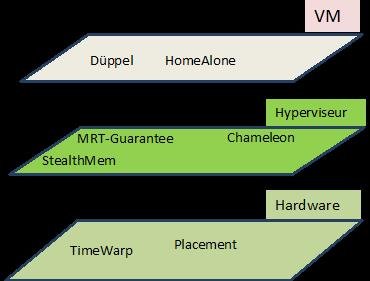
\includegraphics[scale=0.5]{couche.jpg}          
      \caption{\it Répartition des contremesures}
\end{figure}  
\chapter{Approche multicouche} \newline{}

Dans cette partie nous présenterons et évaluerons la nouvelle approche qu’est l’approche multicouche. Tout mécanisme de sécurité se basant sur des hypothèses claires, notre modèle de sécurité est alors le suivant. Notre hyperviseur est supposé  sécurisé, les mécanismes d'exécution simultanée  et de déduplication de mémoire sont désactivés. L’attaquant n’a aucune connaissance des plateformes et des logiciels qu’exécutent les éventuelles victimes. Le seul moyen d’attaque pour un attaquant est l’étude de l’activité du cache.

\section{Algorithme de détection}
Pour se protéger contre les attaques par canaux auxiliaires, il faut bien sûr  au préalable les détecter. Ainsi, nous proposons un nouvel algorithme de détection. Rappelons qu’une attaque par canaux auxiliaires  se fait par la mesure de l’activité d’une victime dans le  cache par un attaquant. Un attaquant voulant faire ce type d’attaque passera la grande partie de son temps d’exécution sur le processeur à faire des mesures en exécutant continuellement des instructions de mesure (instruction rdtsc sur des architectures x86).\newline

Par ailleurs il faut savoir qu’une instruction \textbf{ rdtsc a 14 cycles de latence}. On a alors introduit deux nouveaux paramètres \textbf{cpu-access} et\textbf{ nrdtsc}. La variable cpu-access est un compteur du nombre d’accès d’un processeur virtuel (VCPU) au processeur tandis que la variable nrdtsc matérialise le nombre d’utilisation de la fonction rdtsc par un processeur virtuel dans une machine virtuelle. En outre, de base, les instructions  comme  l’instruction rdtsc lancées par des machines virtuelles au travers de l’hyperviseur \textbf{(KVM)} ne sont pas toutes émulées. Nous avons donc à cet effet pu déterminer le nombre d’appel de la fonction rdtsc en les \textbf{ émulant} et les \textbf{interceptant}. Ainsi puisque l’attaquant préempte régulièrement la victime lors d’une attaque PRIME AND PROBE, à un moment donné lorsqu’il reprend la main du processeur,  l’algorithme vérifie le nombre de fois que l’attaquant a eu accès auparavant au processeur. Deux cas de figure se présentent:

\begin{enumerate}
 \item Si cette valeur est supérieure à deux on peut penser que ce vcpu est  en train d’effectuer une attaque prime and probe. On vérifie alors que le nombre d’appels système rdtsc exécutés pendant la dernière
  exécution de celui-ci en évaluant la variable nrdtsc. On effectue la multiplication de cette valeur par 14. On compare ainsi la valeur obtenue à un seuil critique préalablement déterminé en fonction des paramètres d’ordonnancement. Si cette valeur est supérieure à ce seuil on déclenche une alerte stipulant que  la VM ayant ce  Vcpu est potentiellement une victime
 \item Sinon on ne fait rien
\end{enumerate}
on a donc l'algorithme suivant:
% % % % 
% % % % \begin{algorithm}
% % % % \caption{Détection d'un potentiel attaquant}
% % % % \begin{algorithmic} 
% % % % \RETURN Booléen  
% % % % \Function{changement}
% % % % {\Type{v}{vcpu}}{Booléen}
% % % % {
% % % % \Type{resultat}{entier}
% % % % 
% % % % \IF{$v.cpu_access > 2$ \vee}
% % % % \STATE $resultat \leftarrow 1*14*v.nrdtsc$
% % % % \IF{$resultat \geq seuil$ }
% % % % \STATE $attaquant \leftarrow vrai$
% % % % \PRINT v est un potentiel attaquant
% % % % \ENDIF
% % % % \ENDIF     
% % % % }
% % % % \end{algorithmic}   
% % % % \end{algorithm}

 Notre algorithme est intuitivement réaliste et particulièrement simple à mettre en œuvre.

\section{Architecture de protection}

Comme nous l’avons dit plus haut, une meilleure sécurité nécessite de  prévoir l’attaque dans la totalité et de fournir une contremesure plus générale et fonctionnant de manière  autonome.  Ainsi, pour assurer une protection de bout en bout, nous proposons l’architecture de la figure 6-A ci-dessus. Les éléments constituant cette architecture sont les suivants:
\begin{enumerate}
 \item C'est là où l'algorithme est exécuté
 \item L'agent de détection
 \item Le Framework de protection
 \item L'agent de réaction
\end{enumerate}
L’agent de détection fonctionne conformément à l'algorithme de détection de la section précédente.  Dès que  celui-ci détecte un éventuel attaquant il en informe son agent racine  situé dans le Framework de protection (typiquement VESPA) qui est chargé de  transmettre l’alerte au composant de prise de  décision.  Une fois celui-ci informé, il s’ensuit la prise de décision. Celui-ci transmet la décision de réaction au composant de réaction. Celui-ci se charge donc d’assurer la mise en œuvre des contremesures dans les différentes couches de l’infrastructure. On a alors une boucle autonome de détection et de réaction au travers les différentes couches des plateformes de cloud computing.

\begin{figure}[h!]
      \centering 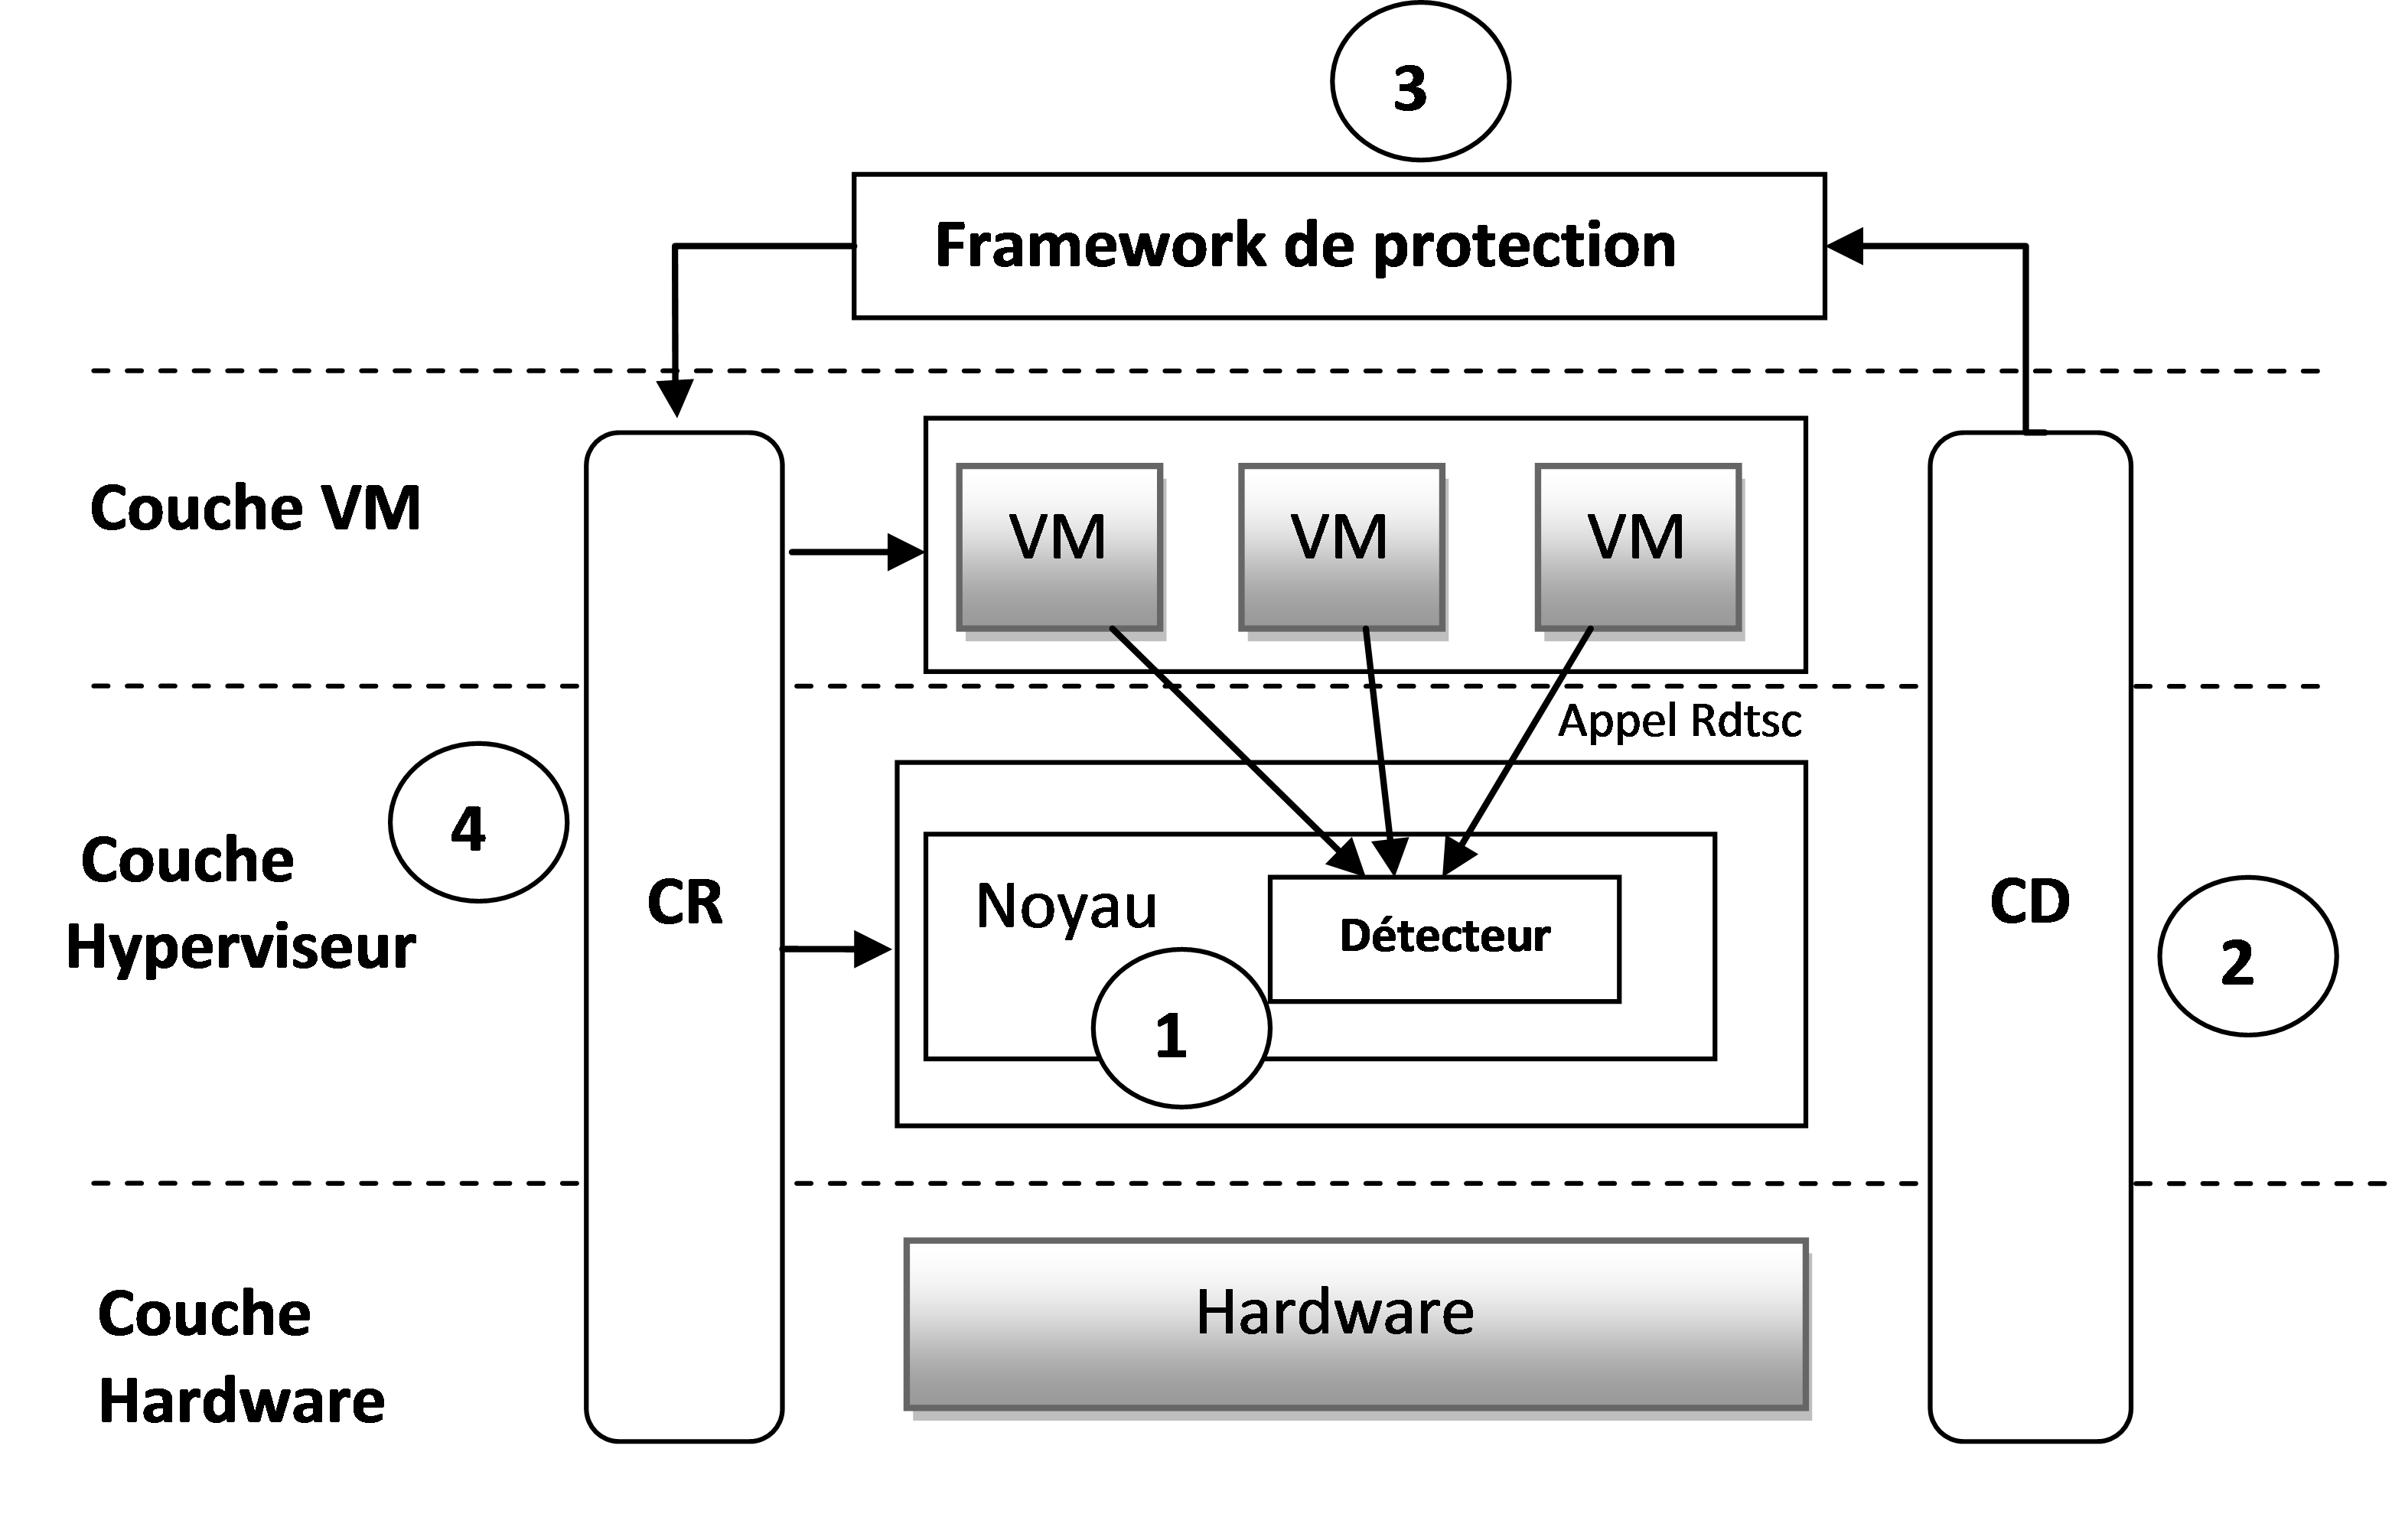
\includegraphics[scale=0.15]{framework.png}          
      \caption{\it Architecture de protection}    
\end{figure}  

    
  
      



    






%%% Local Variables: 
%%% mode: latex
%%% TeX-master: "rapportM2R"
%%% End: 
